\chapter{Programmierung}
\section{Attribute Fahrzeug}
\textbf{Schwierigkeit:} Welche Eigenschaften müssen einem Auto übergeben werden damit eine realistische Simulation möglich ist?
\begin{addmargin}[25pt]{0pt}
	\item \textbf{Lösungsansatz:} Beim Erstellen erhält das Auto eine Position und eine Geschwindigkeit. Die Position besteht aus einer Meteranzeige, wo auf der Strecke es sich aufhält und einer Abfrage auf welcher Spur es sich befindet. Zudem hat es die Möglichkeit zu beschleunigen bezeihungsweise zu bremsen und kann die zugelassene Höchstgeschwindigkeit abfragen. Die Länge jedes Fahrzeugs beträgt 4,5\,m. Das bedeutet, dass LKWs in der Simulation nicht betrachtet werden.\\
\end{addmargin}

\section{Visualisierung}
\textbf{Schwierigkeit:} Wie lässt sich das Reißverschlussverfahren am besten simulieren?
\begin{addmargin}[25pt]{0pt}
	\item \textbf{Lösungsansatz:} Für die Simulation wurde Slick verwendet, da alle Gruppenmitlieder schon Erfahrungen mit Java gesammelt haben und Slick bereits eine graphische Oberfläche für Java besitzt, auf die zugegriffen werden konnte. Somit konnte gleich mit der Implementierung des Reißverschlussverfahren begonnen werden und es musste nicht erst eine graphische Umgebung erstellt werden. Um einen leichteren Einstieg in Slick zu erhalten,wurde ein bereits existierendes Spiel namens "'UfoInvasion"' benutzt, um zu überprüfen, ob Slick auf allen Computern läuft. Daraufhin wurde ein neues Programm geschrieben, in dem lediglich die Slick-Library übernommen wurde. \\
\end{addmargin}
\textbf{Schwierigkeit:} Wie sollte die Fahrbahn aufgebaut sein?
\begin{addmargin}[25pt]{0pt}
	\item \textbf{Lösungsansatz:} Wir betrachten eine Fahrbahnlänge von 1200\,m. Die Länge wurde gewählt, da sie lang genug ist, um die Auswirkungen des Reißverschlussverfahren zu beurteilen, zugleich aber nicht zu groß, damit man noch die einzelnen Autos erkennen kann. Sollte man einen kleineren Abschnitt betrachten wollen, gibt es auch die Möglichkeit heranzuzoomen.\\
\end{addmargin}
\textbf{Schwierigkeit:} Was für visuelle Eigenschaften muss das Auto besitzen?
\begin{addmargin}[25pt]{0pt}
	\item \textbf{Lösungsansatz:} Um die Handlung jedes einzelne Auto zu erkennen, haben wir den Autos Bremslichter und Blinker gegeben. Damit man diese Aktionen auch bei sehr klein abgebildeten Fahrzeugen erkennt, blinkt außerdem die Umrandung. Zudem zeigt die Fahrzeugfarbe den Fahrstyle an. Der aggressive Fahrer ist durch rosa, der neutrale durch blau und der passive durch grün gekennzeichnet.\\
\end{addmargin}

\begin{figure} %Abbildung Fahrzeugtypen: Aggressiv, Neutral, Passiv
\begin{subfigure}{0.1\linewidth}
		\centering
		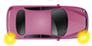
\includegraphics[width=\linewidth]{images/indicating_a}
		\label{fig:indicatinga}
\end{subfigure}
\begin{subfigure}{0.11\linewidth}
	\centering
	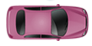
\includegraphics[width=\linewidth]{images/normal_a}
	\caption*{Aggressiv}
	\label{fig:normala}
\end{subfigure} 
\begin{subfigure}{0.1\linewidth}
		 \centering
		 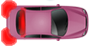
\includegraphics[width=\linewidth]{images/breaking_a}
		 \label{fig:breakinga}
\end{subfigure} 
\begin{subfigure}{0.1\linewidth}
		\centering
		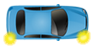
\includegraphics[width=\linewidth]{images/indicating_n}
		\label{fig:indicatingn}
\end{subfigure} 
\begin{subfigure}{0.11\linewidth}
	\centering
	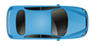
\includegraphics[width=\linewidth]{images/normal_n}
	\caption*{Neutral}
	\label{fig:normaln}
\end{subfigure} 
\begin{subfigure}{0.1\linewidth}
	\centering
	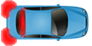
\includegraphics[width=\linewidth]{images/breaking_n}
	\label{fig:breakingn}
\end{subfigure} 
\begin{subfigure}{0.1\linewidth}
\centering
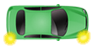
\includegraphics[width=\linewidth]{images/indicating_p}
\label{fig:indicatingp}
\end{subfigure}  
\begin{subfigure}{0.11\linewidth}
			\centering
			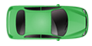
\includegraphics[width=\linewidth]{images/normal_p}
			\caption*{Passiv}
			\label{fig:normalp}
\end{subfigure} 
\begin{subfigure}{0.1\linewidth}
	\centering
	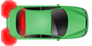
\includegraphics[width=\linewidth]{images/breaking_p}
	\label{fig:breakingp}
\end{subfigure}
\caption{Fahrzeugtypen: Aggressiv, Neutral, Passiv}
\label{fig:fahrzeug}
\end{figure}

\section{Spawner}
\textbf{Schwierigkeit:} Wie schafft man es einen realistischen Verkehrsfluss zu erzeugen, um den Eingangsverkehr in das Simulationsgebiet zu Simulieren.
%Wie schafft man es Fahrzeuge zu erzeugen, die mit einem realistischen Verkehrsverhalten an das Stauende fahren.
\begin{addmargin}[25pt]{0pt}
	\item \textbf{Lösungsansatz:} Da die Simulation lediglich ein beschränktes Gebiet betrachten, ist es notwendig das in das Gebiet hineinfließende Verkehrsverhalten möglichst realistisch darzustellen. Hierbei wird die Realität auf folgende Aspekte beschränkt: 
	\begin{itemize}
		\item der Sicherheitsabstand wird eingehalten
		\item Fahrzeuge werden mit ähnlicher Geschwindigkeit erzeugt
		\item Fahrzeuge fahren links schneller, aufgrund des rechtsseitigen Überholverbots
		\item auf der rechten Fahrspur gibt es eine höhere Verkehrsdichte
	\end{itemize}
	Um ein neues Fahrzeug in die Simulationumgebung hinzuzufügen wird eine normal verteilte Zufallszahl gewählt, welche den Zeitpunkt für die Erzeugung eines Autos beschreibt. Erwartungswert und Standardabweichung verhalten sich umgekehrt proportional zur gewünschten Verkehrsdichte. Ist dieser Zeitpunkt erreicht, wird anhand der vorraus fahrenden Autos der vorhandene Platz berechnet. Damit ein Auto erzeugt werden kann, muss der vorhandene Platz mindestens dem Sicherheitsabstand betragen. Zusätzlich wird die Geschwindigkeitsbeschränkung für das erzeugte Auto berechnet. Diese Geschwindigkeitsbeschränkung ist so definiert, dass das Auto noch genug Zeit zum Bremsen hat, um einen Unfall zu vermeiden. Eine ähnliche Geschwindigkeit wir dadurch gewährleistet, dass die Geschwindigkeit in Abhängigkeit der derzeitigen Verkehrsgeschwindigkeit berechnet wird, jedoch die Geschwindigkeitsbeschränkung nicht überschreiten darf. Zusätzlich müssen Fahrzeuge die auf der linken Spur erzeugt werden mindestens die Spurgeschwindigkeit der rechten Spur besitzen, um das rechtseitige Überholen zu verhindern.
	%TODO Fahrertypen??
	
%	Hierzu muss eine Vielzahl von Aspekten beachtet werden. So zeichnet sich der Verkehrsfluss unter anderem dadurch aus, dass die einzelnen Autos genügend Abstand halten, sowie eine ähnliche Geschwindigkeiten besitzen. Ebenfalls wichtig ist es, die Verteilung auf den Fahrbahnen realitätsnah darzustellen.
%	Dazu ist es wichtig die Verkehrsdichte zu berücksichtigen. Hierzu wurde eine normal verteilte Zufallszahl gewählt, welche den Zeitpunkt für die Erzeugung nächsten Autos beschreibt. Erwartungswert und Standardabweichung verhalten sich umgekehrt proportional zur gewünschten Verkehrsdichte.	
%	Ist dieser Zeitpunkt erreicht, wird anhand der fahrenden Autos der vorhandene Platz, sowie die maximale Geschwindigkeitsbeschränkung des Autos berechnet. Zu verhindern gelten Geschwindigkeiten, bei denen das Auto nicht mehr rechtzeitig bremsen kann. Ist genügend Platz vorhanden, wird ein neues Auto mit zufällig gewähltem Fahrertyp(aggressiv, neutral, passiv) erzeugt. Als Initialwerte werden gleichmäßige Anteile aller Typen angenommen.
%	Die Initialgeschwindigkeit des Fahrzeugs berechnet sich in Abhängigkeit der derzeitigen Verkehrsgeschwindigkeit. Die Wahrscheinlichkeiten der einzelnen Fahrertypen können während der Simulation geändert werden. Im Anschluss wird das Auto erzeugt und ein neues deltaT für das nächste Auto. Dies wir für jede Bahn durchgeführt.
%
%	Mithilfe dieses Verfahrens ist es möglich zufällig Autos auf beiden Fahrbahnen zu erzeugen, ohne dass diese Aufgrund zu hoher Initialgescshwindigkeiten aufeinander auffahren. Dies spiegelt allerdings kein realistisches Verkehrsbild wieder, da noch nicht geregelt wird, dass die Geschwindigkeit der linken Bahn im fließenden Verkehr in der Regel höher ist als die der rechten Fahrbahn (Überholverbot rechts%TODO
%	). Hierfür wurde eingeführt, dass zum einen auf der linken Bahn mindestens so schnell gefahren werden muss wie auf der rechten Bahn, falls dies in der derzeitigen Verkehrslage möglich ist, sowie dass die rechte Bahn bei nicht stockendem linken Verkehr langsamer fahren muss(erzeugt wird),als die rechte.
%	
%	Des weiteren galt es die Mindestgeschwindigkeit der Autos zu regeln, da es aufgrund der zufälligen Generierung zu sehr hohen ausschlägen nach sowohl unten, wie auch oben kommen kann. 
%	Hierfür wurde lediglich eine unterer Grenzwert der Geschwindigkeit in abhängigkeit der Bahngeschwindigkeit eingeführt. Bei entsprechend niedriger Bahngeschwindigkeit ist es dadurch immernoch möglich sehr langsame Autos zu erzeugen.
%	
%	Neben der Initialgeschwindigkeit, werden den Autos ebenfalls eine initial Zielgeschwindigkeit zugewiesen(Berechnung über normalverteilte Zufallszahlen), auf welche sie gerne beschleunigen würden, falls der Verkehr es zulässt. Dies war wichtig, da es ansonsten zu Problemen kam, wenn ein Auto direkt mit sehr niedriger Geschwindigkeit erzeugt wird(zum beispiel direkt am Stauende), da diese Autos nach auflösung des Staus auf ihrer niedrigen Geschwindigkeit geblieben sind, anstatt auf ein angemessenes Tempo zu beschleunigen.
	
	%Bevor ein neues Fahrzeug gespawnt werden kann, müssen mehrere Bedingungen erfüllt sein. Dazu gehört zu aller erst der Sicherheitsabstand. Dieser wird aus der Geschwindigkeit des vorrausfahrenden Fahrzeuges und dem Tempolimit errechnet. Erst wenn gewährleistet ist, das genug Sicherheitsabstand existiert wird der Spawner freigegeben. Je nach gewünschter Verkehrsdichte spawnt dann nach einer gewissen Zeit ein neues Auto. Dieses Auto besitzt eine zufällige Geschwindigkeit. Diese Geschwindigkeit orientiert sich am vorrausfahrendem Fahrzeug. So liegt der Erwartungswert der Geschwindigkeit bei der Bahngeschwindigkeit des Vordermann plus ein Drittel der Differenz der Höchstgeschwindigkeit und der Bahngeschwindigkeit. Zudem ist geregelt, das Autos die auf der linke Spur erzeugt werden mindestens 80\% der aktuellen Bahngeschwindigkeit besitzen und auf der rechten mindestens 60\%. Dies verhindert das ein viel zu langsames Auto spawnt, was zum einen Realitätsfern wäre und zum Andern den Verkehrsfluss unnötigerweise verlangsamt.\\
\end{addmargin}

\section{Bedienung}
\textbf{Schwierigkeit:} Wie erhält man eine benutzerfreundliche Bedienungsoberfläche, bei der man möglichst viele Variablen verändern kann.
\begin{addmargin}[25pt]{0pt}
	\item \textbf{Lösungsansatz:} Die Steuerung über Eingabefelder hat sich als am Benutzerfreundlichsten herausgestellt. Hier hat der Benutzer die Möglichkeit auf Skalierung, Zeitraffer, Verkehrsdichte, sowie den Anteil der Fahrertypen, Einfluss zu nehmen. Um Fehler zu vermeiden, werden nur sinnvolle Eingaben berücksichtig.\\ 
	Mithilfe der Skalierung kann man an die Verengung herranzoomen. Bei der Standardeinstellung von 0.09 wird der komplette Simulationsbereich betrachten.\\ 
	Der Zeitraffer dient dazu Langzeitentlicklungen schneller darstellen zu können. Hierbei ist jedoch zu beachten, dass durch die Verwendung des Zeitraffers die Abtastrate sinkt. Dadurch ist die Genauigkeit nicht mehr gewährleistet. Bis zur fünffachen Geschwindigkeit sind die Ergebnisse noch recht genau, bei einer schnelleren Betrachtung dient das Ergebnis lediglich als Annäherung.\\
	Durch die Verkehrsdichte kann man die Erzeugungswahrscheinlichkeit von Fahrzeugen verändern. Die Verkehrsdichte hat massgeblichen Einfluss auf die Effektivität des Reißverschlussverfahren. Diesen Einfluss kann der Benutzer anhand der ausgegebenen Durchschnittsgeschwindigkeit, der Eingangsverkehrsdichte, sowie der Ausgangsverkehrdichte ablesen.\\
	Zu guter letzt kann der Benutzer noch den Anteil der Fahrertypen variieren. Standardmäßig gibt es 33\% aggressive (rosa), 33\% passive (grün) und 33\% neutrale Fahrer (blau). Die Anteile addieren sich immer zu 100\% auf, wobei die aggressiven und passiven Anteile durch Eingabefelder veränderbar sind und der neutrale Fahrer die restlichen Anteile bekommt.\\
	Solle der Benutzer zusätzliche Informationen zu den jeweiligen Autos bekommen wollen, kann er durch Betätigung des "'D"' auf der Tastertur sich zu jedem Auto dessen ID, die derzeitige Geschwindigkeit, sowie die Beschleunigung anzeigen lassen. Diese Funktion wurde zum Debuggen erstellt, wodurch kein großer Wert auf die Lesbarkeit gelegt wurde und somit sich die Datenausgaben überlagern können.\\
\end{addmargin}

\section{Fahrer}
\textbf{Schwierigkeit:} Es gibt in der Realität viele unterschiedliche Fahrertype. Jeder Fahrer hat einen individuellen Fahrstyle. Diese lassen sich häufig in Kategorien wie zum Beispiel aggressive oder passive Fahrer einordnen. Ganz ohne die Unterscheidung von Fahrertypen wäre die Simulation nicht Realitätsgetreu.
\begin{addmargin}[25pt]{0pt}
	\item \textbf{Lösungsansatz:} Die Programmierung von sehr vielen Fahrertypen ist zeitaufwendig und alle psychologischen Aspekte sind nicht darstellbar. Es wurden drei Fahrertypen imlementieren: Den Aggressiven (rosa), den Neutralen (blau) und den Passiven(grün). Diese drei Fahrertypen unterscheiden sich darin, wie großen Sicherheitsabstand sie einhalten, mit welcher Geschwindigkeit sie erzeugt werden, wie stark der Fahrer abbremst sobald das vorrausfahrende Fahrzeug bremst und wie sie sich beim Einsortieren verhalten. So hat der aggressive Fahrer eine deutlich höhere Wahrscheinlichkeit, dass er mit einer erhöhten Geschwindigkeit erzeugt wird, als der passive oder neutrale Fahrer. Zudem nutzt der aggressive Fahrer jede noch so kleine Lücke die sich bei der Verengung ergibt. Der Passive hingegen lässt einen deutlich größenen Sicherheitsabstand zum vorrausfahrenden Fahrzeug und hat einen höheren "Panikfaktor", welcher bewirkt, dass er sobald vorne gebremst wird, auch stark abbremst.\\
	Um die Simulation realitätsgetreuer zu machen besitzt jeder Fahrer über eine Reaktionszeit von 250/,ms. Dadurch bremsen nicht alle Fahrzeuge gleichzeitig sondern erst wenn der Vordermann auch bremst.\\
\end{addmargin}